\section{GPU硬件结构与CUDA编程模式}
本文中的并行算法均在Nvidia GPU上通过CUDA编程模式实现,为了帮助理解本文的并行算法设计思路,我们首先介绍GPU的硬件架构和CUDA 编程模型。
%%they are a single section
\subsection{CPU与GPU}
\begin{figure*}
\setlength{\belowcaptionskip}{-0.5cm}
  \begin{center}
    {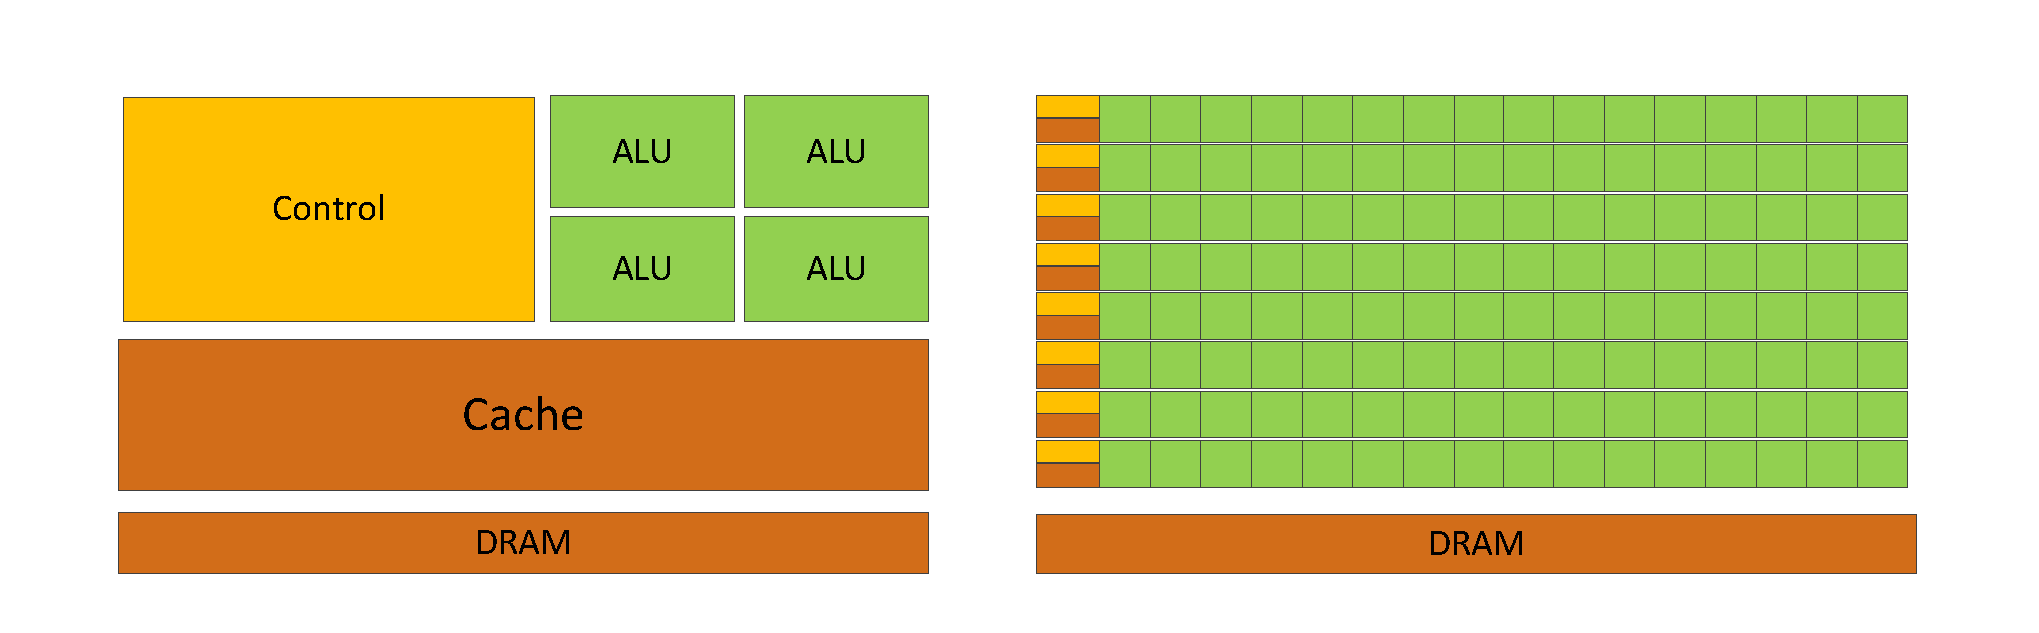
\includegraphics[width=1 \textwidth]{figures/GPU&CPU.pdf}}
    \end{center}
  \caption{{\footnotesize{drk}}}
  \label{drk}
\end{figure*}
\subsubsection{CPU与GPU区别}
上图为CPU和GPU的架构比较,可以看到,CPU和GPU的差异主要有两点 第一,GPU的ALU单元远远多于CPU;第二,GPU 每个核心可用的逻辑控制单元和缓存相对CPU要少很多。CPU 上大面积晶体管是逻辑控制单元和缓存单元,这是因为CPU的设计需要兼容多方面的应用,比如在桌面应用中就具有大量的分支控制操作和存储操作,而真正的数值计算操作却很少,所以CPU 上具有大量的逻辑控制相关的实现,比如分支预测(Branch Prediction),乱序执行(OoO 来满足这些分支控制需求,同时增加缓存大小来加速存储过程,但是这样的设计也使得留给CPU上的计算单元的晶体管面积较少,浮点计算能力较差,现在CPU为了弥补其计算能力得不足,产商常常在同块芯片上集成多个CPU 核心,组成多核处理器,但是这样的设计并不能提高晶体管的利用率。
GPU最初被设计来进行图像渲染,图像渲染具有高度的并行性,而且大部分操作是浮点计算操作,逻辑控制较少,所以GPU在设计上采用简化控制单元,增加计算单元的设计思想,这使得GPU在进行大规模浮点运算的任务时大大优于CPU的执行速度。
\subsubsection{CPU+GPU异构计算模型}
通过上面的分析可以看到GPU适用于线程数目多,浮点计算密集和逻辑较简单的并行任务,而CPU更加适应与串行任务和分支较多,计算较少的任务。所以在实际中,常常把CPU 和GPU结合起来,使用CPU和GPU两个部分协作共同完成并行计算任务,在这些并行任务中,CPU主要用于逻辑控制部分,而GPU 作为一种设备被CPU控制调用来做并行计算工作,这种协同工作模型被称为CPU+GPU 异构计算模型。
如图,所示为CPU+GPU异构计算结构示意图,GPU和CPU通过PCI总线进行连接。CPU调用GPU 执行一共需要以下步骤:
\newline
1.把输入数据从CPU主机内存拷贝到GPU的主存DRAM中。\newline
2.把执行程序加载到GPU上然后执行。\newline
3.GPU上的程序执行需要从主存中读取数据,为了加快访问速度,数据将通过L1 cache和L2 cache进行缓存。\newline
4.GPU上程序执行完毕,将结果写在GPU主存中,这时需要将结果重新拷贝会CPU主机端进行处理。\newline
\begin{figure*}
\setlength{\belowcaptionskip}{-0.5cm}
  \begin{center}
    {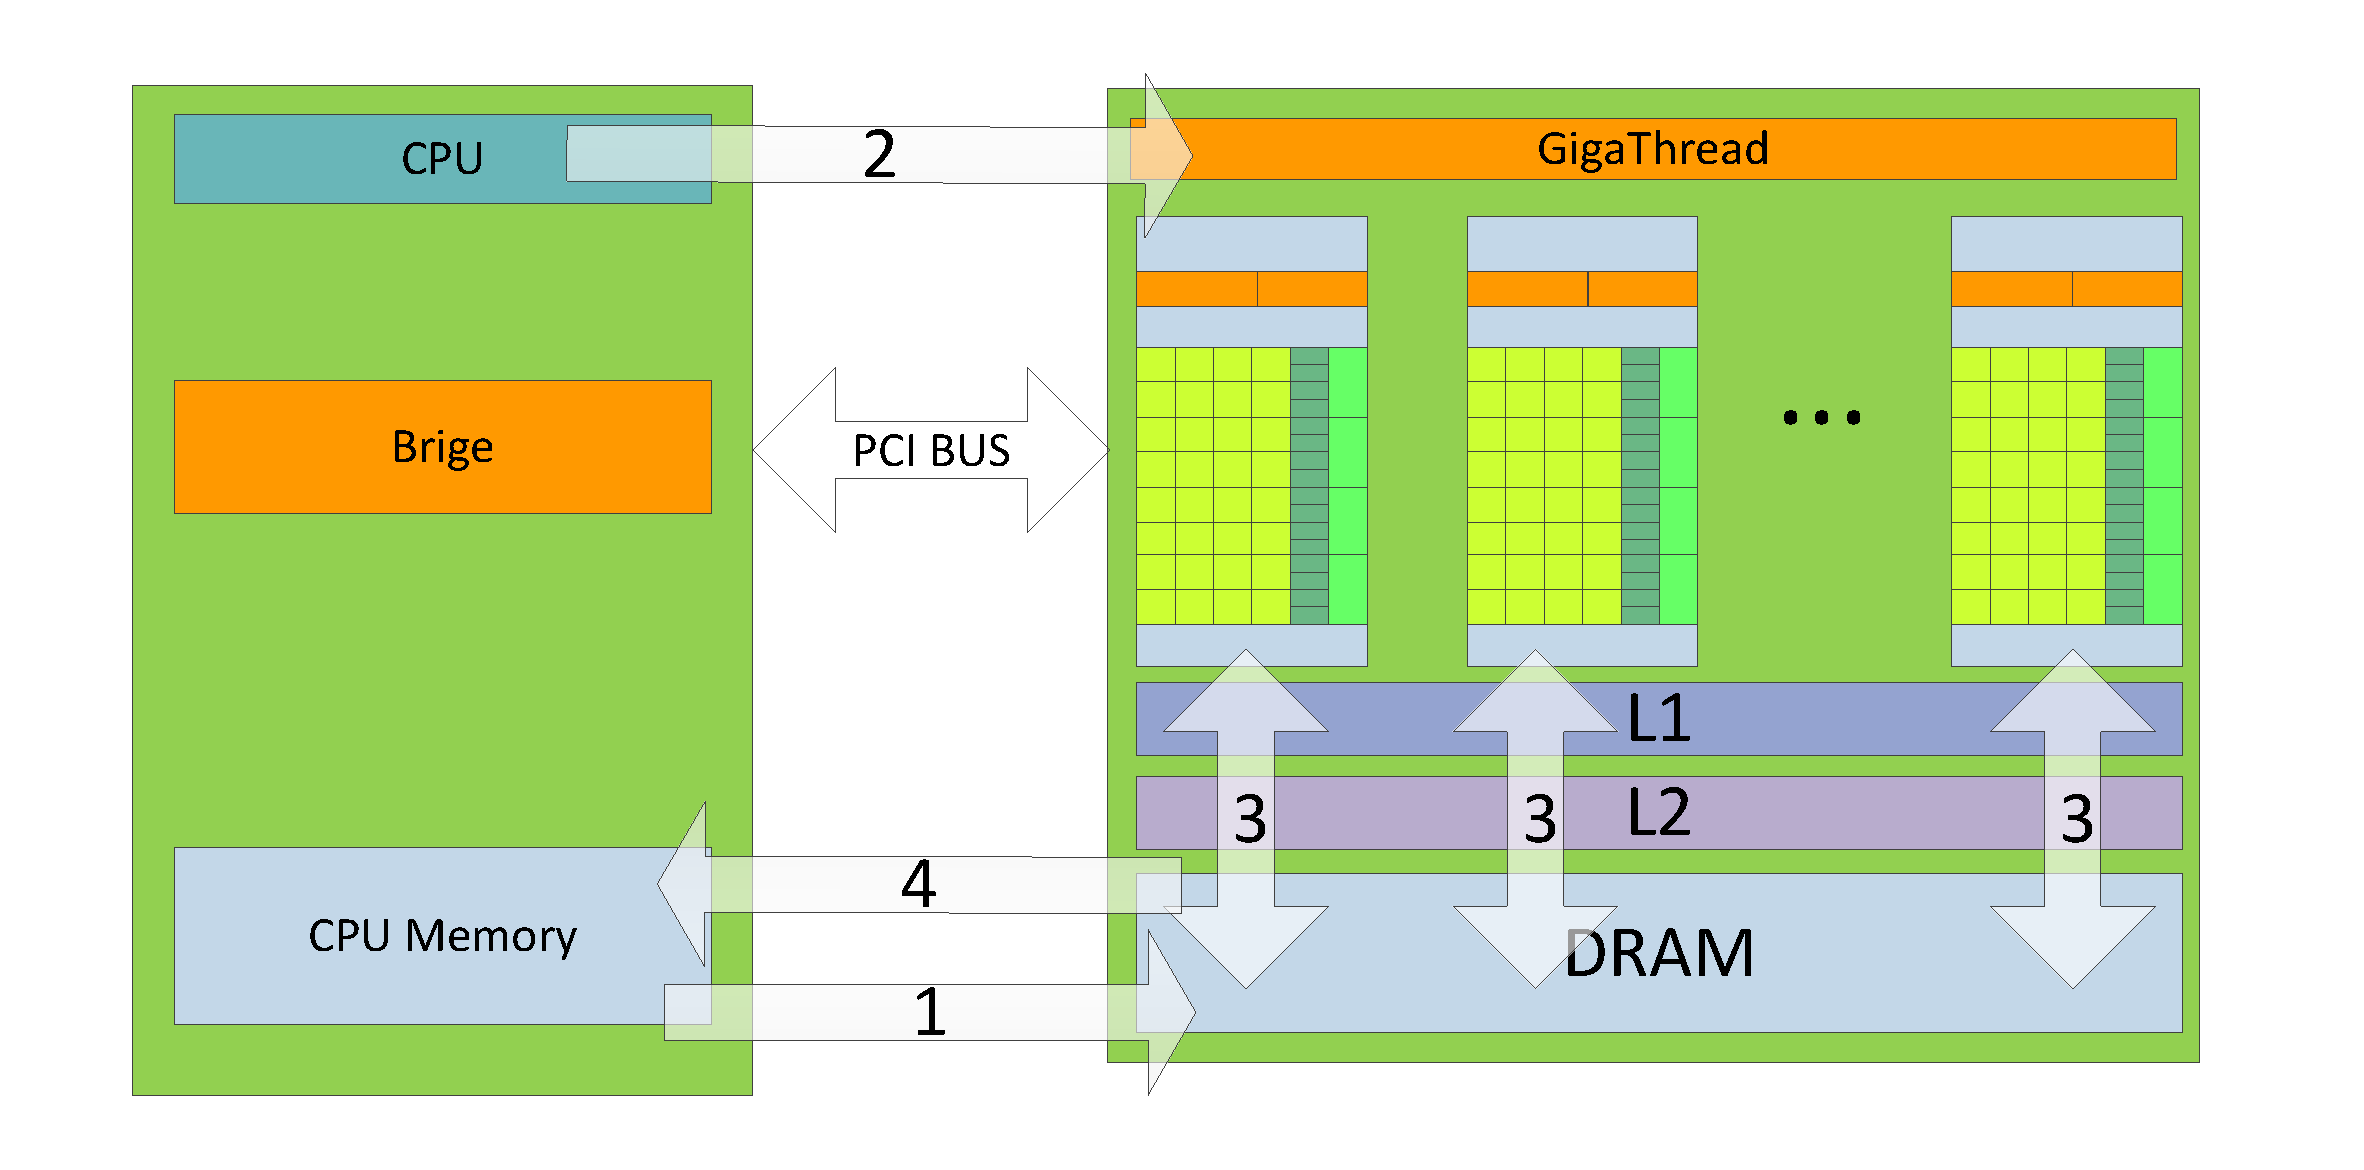
\includegraphics[width=1 \textwidth]{figures/yigou.pdf}}
    \end{center}
  \caption{{\footnotesize{drk}}}
  \label{drk}
\end{figure*}
\subsection{GPU硬件架构}
虽然GPU相对于CPU在并行算法方面有很多优势,但是,由于GPU的出现是为了加速图形渲染问题,当想要使用GPU进行图形学之外的通用计算时,我们需要将通用问题转换为图形学问题,并且通过OpenGL或者DirectX等APU来访问GPU,这对普通的开发人员提出了更高的要求,限制了GPU程序的设计自由度,使得GPU通用计算变得困难,
为了简化GPU的通用计算,降低开发难度。2007年6月,NVIDIA推出CUDA (Compute Unified Device Architecture,统一计算设备架构)。CUDA 不需要借助与其他的图形学API,CUDA采用简单的类c语言进行开发,这使得开发人员可以很容易的进行GPU 的开发。但是,为了设计出高效率的GPU并行程序,开发人员需要掌握GPU架构上的相关知识。
我们以kepler架构为例子来介绍GPU的硬件架构。图1位kepler的GPU架构模型细节,kepler架构包含两个部分,流处理器阵列(core 部分)和存储系统(memory)部分,kepler架构中的GPU上一共包含15个流多处理器(SM),所有流多处理器共享一个L2缓存。
\subsubsection {流处理器}
我们看到GPU中主要组成部分是SM,一个SM(stream mutiprocessor)中含有大量的sp,sp(stream processor)为GPU的计算核心,又称为流处理器,sp 是最基本的处办理单元,指令和任务最终都是sp上处理的,我们可以将在一个SP上执行的流看做一个独立的线程(thread),如果一个GPU中有更多的SM,一个SM中有更多的sp,那么就意味着这个GPU 在相同的时间内可以并行处理更多的任务。
\subsubsection{线程束(Wrap)}
warp是SM调度和执行的单位,一个SM中的thread会在物理上被分组成不同的warp,通常一个warp 包含32个thread,同一个warp中的线程执行相同的指令,同一个warp中的线程始终是同步的,也就说同一个warp 中的线程必须等待所有线程都执行完了同一个指令后,才会去执行下一个指令,这样的设计虽然节省了硬件的控制单元的复杂程度,但是也限制了GPU 在处理分支时的并行粒度,如果同一个warp 中的线程出现分支,每个线程执行的分支条件不一样,为了保持同步,不进入分支的空闲sp 也必须等待进入分支的线程执行完毕后才能继续执行,这样使得sp 的利用率下降。\newline
warp作为隐藏延迟的基本调度单元,我们知道GPU 的浮点计算能力很强,但是在一些应用中常常需要进行内存的读写操作,这些访存操作需要大量的时间延迟,从而限制了GPU的浮点计算吞吐量,为了充分利用GPU 上大规模的sp,GPU采用warp 切换来隐藏这些延迟。同一个SM上可以存在多个warp的程序上下文,但是同一时间只能有限个warp 被执行,下图展示了warp上下文的切换过程,假设每个warp执行相同的代码,代码中需要先进行Load 操作,再进行计算操作,Load 操作需要等待4 个时钟周期,而计算操作只需要使用一个时钟周期,W1-W4 表示4个不同的warp 线程组,开始时W1 先执行Load 操作,而load 操作阻塞,这时调度器执行调度将W2 调度到sp 上进行执行,继续阻塞,直到第5个周期,W1的数据已经准备好了可以进行计算操作,当W1 的计算操作结束后,继续切换计算W2,W3,W4。通过这个例子我们可以看到GPU 上的warp切换能够很好得隐藏延迟,提高sp 的利用率。\newline
\subsubsection{存储结构}
GPU中的每个SM中含有一定数量的寄存器,共享内存,常量内存,纹理内存。寄存器用来存储程序执行中的临时变量,同一个SM 中的线程都能够访问共享内存,共享内存的访存速度大大高于主存的访存速度,所以在GPU并行代码设计时,我们常常先把频繁访问的数据提取到共享内存中,以减小延迟。另外,将中间结果存储在共享内存中,以减小对主存的访问,但是共享内存的大小是有限的,在kepler架构中共享内存的大小为64KB。常量内存是用来缓存计算时需要的一些常量,常量内存为只读数据,用常量内存来替换全局内存可以有效地减少内存带宽占用,常量内存大小为48KB。 纹理内存是一种特殊的只读缓存,纹理内存是专门为图形应用程序设计的,在一些特殊的具有大量空间局部性的内存访问模式中能够提升性能并且减少内存流量。\newline
\subsubsection{流多处理器细节}
通过上面对sp,warp和存储器的介绍,我们再分享下kepler架构下的SMX 细节。从图中,可以看到,kepler架构下的SMX中包含192 个单精度的CUDA core,64个双精度的单元(DP unit)和32个SFU(Special Function Unit, 特殊函数单元),32个存储(load/store)单元,其中SFU 用来执行超越函数、插值以及其他特殊运算。Kepler的每个SM 包含4个warp scheduler和8个instruction dispatchers。 Kepler K20X(compute capability 3.5)每个SM可以同时调度64个warp 共计2048个thread,而kepler 架构中一共有15个SMX,也就是说,同一时刻最大可以支持30720个线程在GPU上调度执行,所以GPU的并行能力相当强大。\newline
\subsubsection{执行模型}
GPU采用了SIMT(Single Instruction ,Mutiple Thread)执行模型,SIMT是对SIMD的一种改进。在CPU的SIMD中,向量宽带是受限的,在Intel 的SSE指令集中,一条SSE的指令宽带为128bit,一次可以处理4个单精度浮点数,或者两个双精度浮点数,如果要用SSE指令处理一个单精度浮点数构成的数组,必须将数组按4个一组的方式进行打包,然后才能交给CPU进行处理。但是在CUDA的模型中,我们为相同的指令产生不同的线程,这些线程的数量可以自由设置,在kepler架构中,同一时刻GPU上可以调度执行30720 个线程,这比CPU的SIMD的并行粒度高很多。\newline
\begin{figure*}
\setlength{\belowcaptionskip}{-0.5cm}
  \begin{center}
    {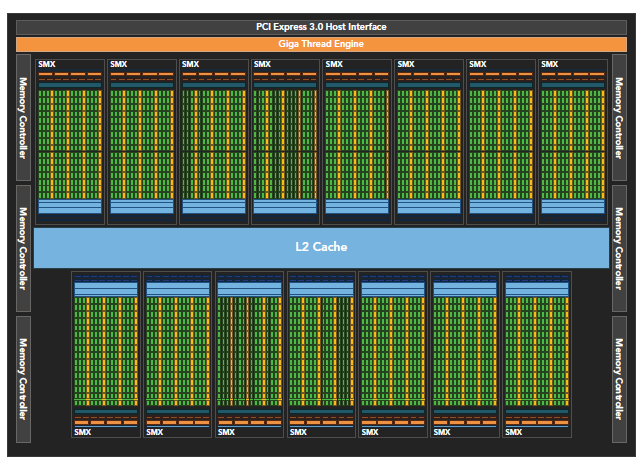
\includegraphics[width=1 \textwidth]{figures/arc.png}}
    \end{center}
  \caption{{\footnotesize{drk}}}
  \label{drk}
\end{figure*}
\begin{figure*}
\setlength{\belowcaptionskip}{-0.5cm}
  \begin{center}
    {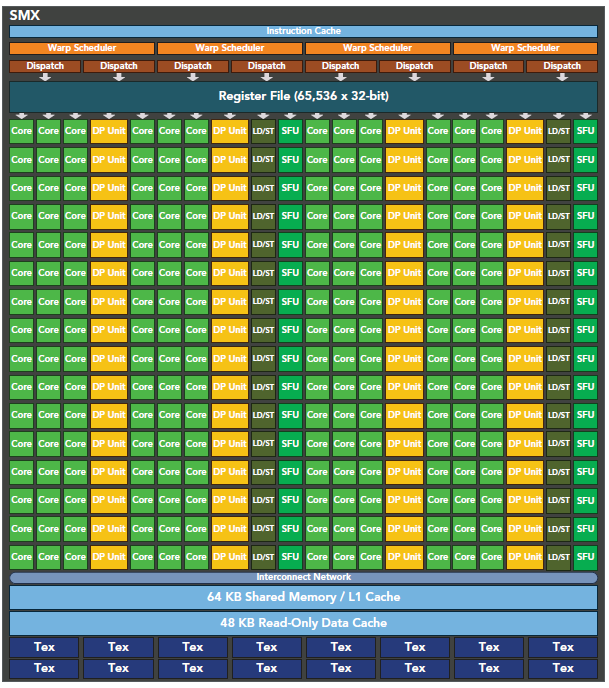
\includegraphics[width=1 \textwidth]{figures/smx.png}}
    \end{center}
  \caption{{\footnotesize{drk}}}
  \label{drk}
\end{figure*}
\begin{figure*}
\setlength{\belowcaptionskip}{-0.5cm}
  \begin{center}
    {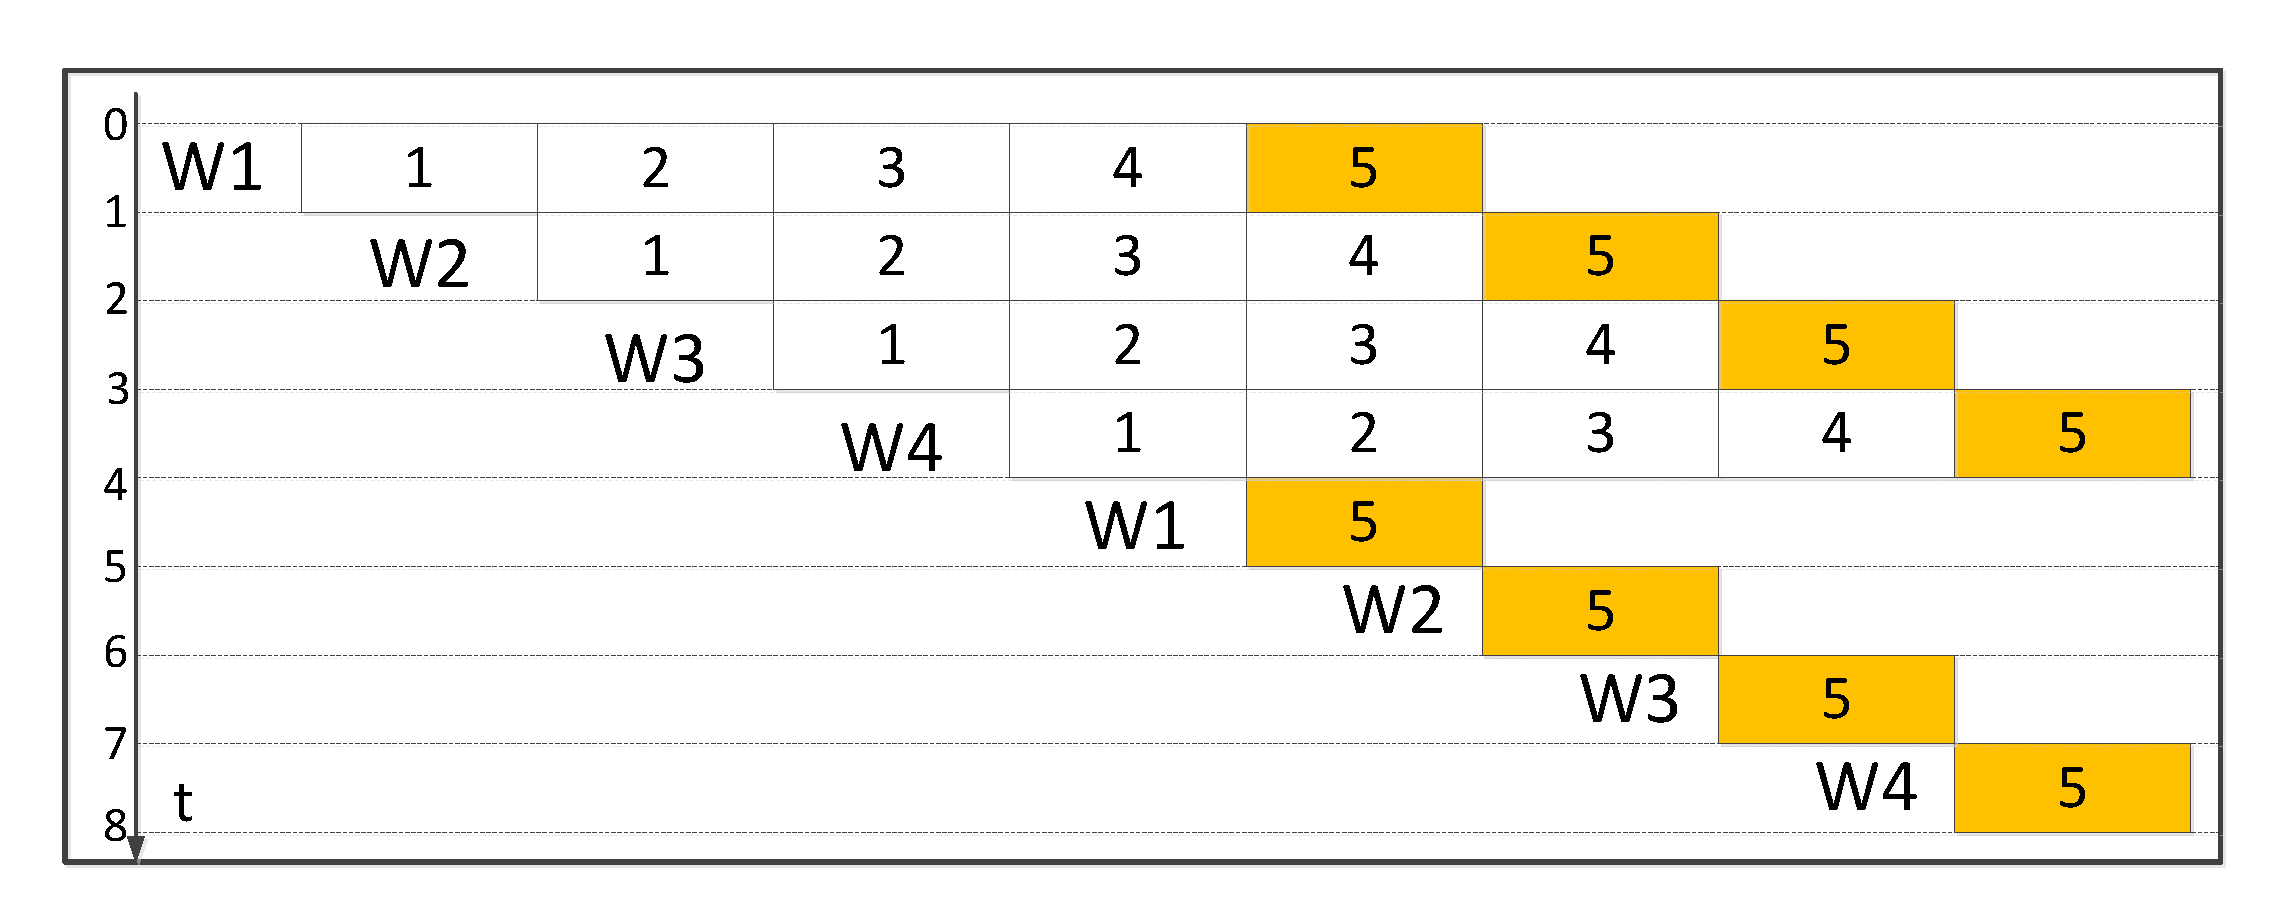
\includegraphics[width=1 \textwidth]{figures/warpsketch.pdf}}
    \end{center}
  \caption{{\footnotesize{drk}}}
  \label{drk}
\end{figure*}
\subsection{CUDA编程模式}
CUDA 是一种CPU和GPU的异构计算模型,CUDA的应用程序被分为两个部分,一部分为主机端的代码,一部分为设备端的代码,主机端的代码在主机CPU 上执行,主机负责调度GPU设备执行设备端代码。一个主机可以对应多个GPU设备,图,展示了CUDA 异步执行流程,CPU通过调用kernel 函数的方式控制GPU 执行并行程序。\newline
\begin{figure*}
\setlength{\belowcaptionskip}{-0.5cm}
  \begin{center}
    {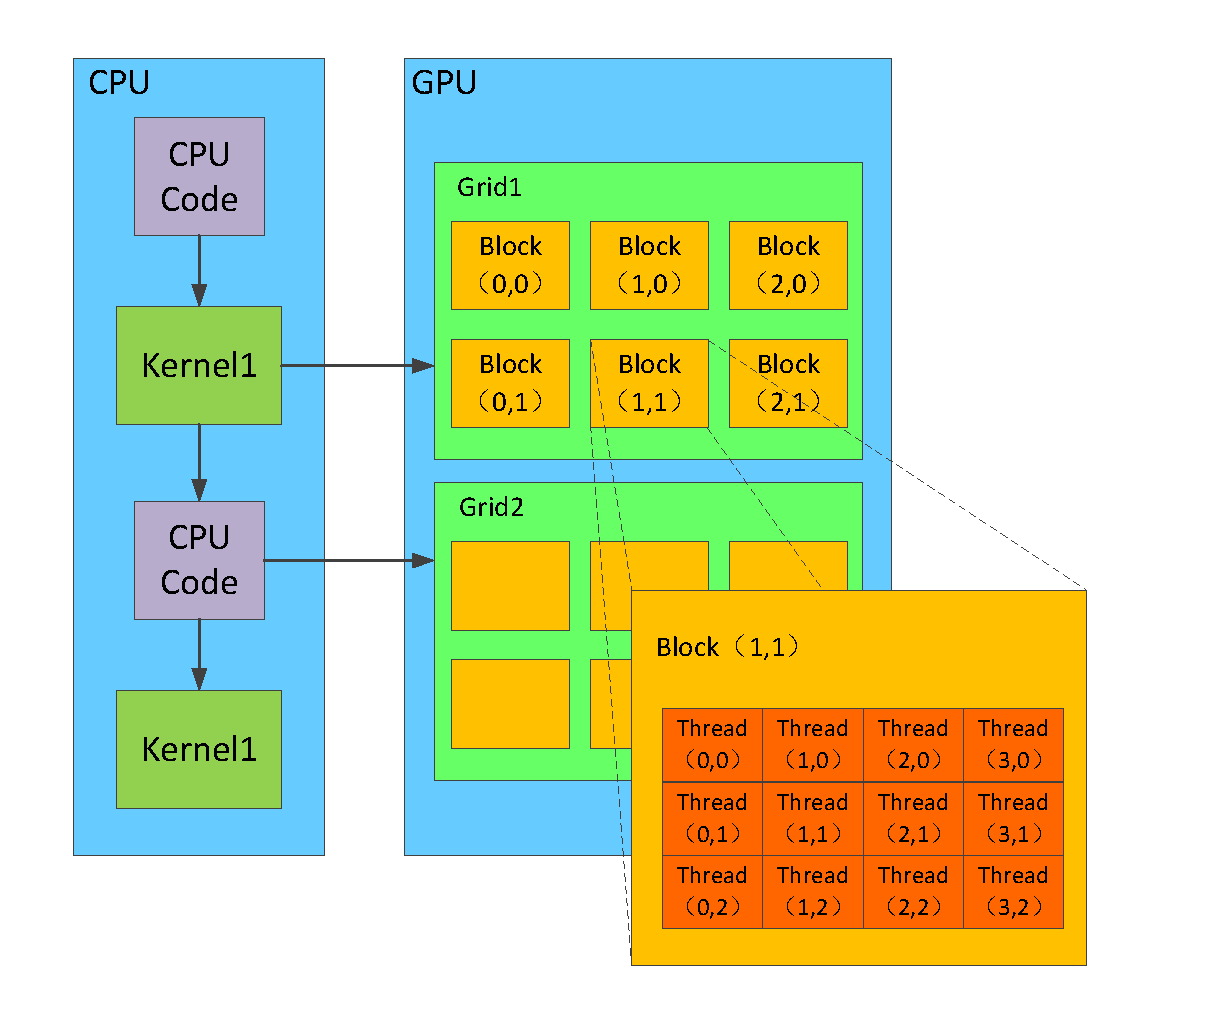
\includegraphics[width=1 \textwidth]{figures/block.pdf}}
    \end{center}
  \caption{{\footnotesize{drk}}}
  \label{drk}
\end{figure*}
\subsubsection{CUD软件线程组织}
一个CUDA的并行程序会以多个thread来执行,在软件层面上,我将数个threads组成一个block,同一个block中的线程又被分成不同的warp,他们只能在同一个SM中执行,同一个block中的线程可以通过调用同步函数(\_\_syncthreads())进行同步,同一个blcok中的线程可以共同访存shared\_memory,通过shared\_memory实习通信。一个kernel函数可以在软件层面上产生大量的线程,这些线程被组织成一个一个的block,如果SM足够,这些block中的线程将被加载到SM 上调度执行,如果SM不足,block需要排队等待其他block完成执行。多个block组成一个Grid,block的维度可以是1-3维,图,展示了一个二维的block组织,每个block有自己的二维标号,同样每个block内部的线程也可以被组织成1-3维,图,展示了一个block内部的thread二维标号。在编写kernel函数时,CUDA 使用blockIDx.x,blockIDx.y,blockID.z三个标号来访问当前线程的block标号,使用threadIDx.x,threadIDx.y,threadIDx.z三个标号来访问当前线程的标号。blockDim.x,blockDim.y,blockDim.z 分别表示block中的thread三个维度的宽度。gridDim.x,gridDim.y,gridDim.z分别表示Grid中的block的三个维度的宽度。\newline
\subsubsection{CUDA C的程序结构}
下图为CPU何GPU的程序结构,在CPU端调用kernel函数之前需要将kernel函数中用到的数据拷贝到GPU上,通常采用函数cudaMalloc()在GPU端分配内存,采用函数cudaMemcpy()将主机上的数据拷贝到GPU端,数据拷贝好后,CPU 端调用kernel函数,kernel 函数被加载到GPU 端进行执行,执行完毕后将数据通过cudaMemcpy()拷贝会主机,下面的伪代码展示了cuda程序的编程框架。\newline
\begin{lstlisting}[language=C],
//`变量声明`
__host__,...,__device__...__global__,
__constant__,__texture__,__shared__
//内核函数原型声明
__global__ void Kernel(args)
{
}
void main(){
    //`在GPU端分配数据内存空间`
    cudaMalloc(&device_data,bytes);
    //`拷贝输入数据到GPU端`
    cudaMemcpy(device_data,host_data);
    //`配置kernel函数,并且发射kernel函数在GPU端执行`
    Kernel<<<configuration>>>(args);
    //`拷贝结果到主机`
    cudaMemCpy(host_data,device_data);
}
\end{lstlisting}
\subsubsection {函数和变量修饰符}
CUDA对c扩展了三种函数声明修饰符:\_\_global\_\_,\_\_device\_\_和\_\_host\_\_,下表对这三种函数函数修饰符进行了介绍,\_\_host\_\_ 修饰的函数和一般的c语言函数一样,只在主机端调用和执行,\_\_global\_\_修饰的是kernel函数,kernel函数在设备端调用,但是在GPU上执行。\_\_device\_\_函数在GPU端由kernel函数或者其他\_\_device\_\_函数调用并且在GPU上执行。\newline
\begin{table}[h]
\centering
\begin{tabular*}{14cm}{@{\extracolsep{\fill}}ccccccccc}
\hline
函数名称& 执行位置& 调用位置\\
\hline
\_\_global\_\_ void kernelFunc()& GPU设备& 主机\\
\_\_device\_\_ float DeviceFunc()& GPU设备& GPU设备\\
\_\_host\_\_ float HostFunc()& 主机& 主机\\
\hline
\end{tabular*}
\end{table}
GPU中的同时执行大量线程,如果这些线程都去访问全局内存,会使得全局访存带宽拥堵,增大延迟,所以GPU中有多种的独特的内存结构,来优化访存模式,设计CUDA程序时需要把程序的内存访问特点和GPU内存架构特点相结合,这样才能设计出高效的GPU代码,为了支持对这些内存结构的操作,CUDA 对c 扩展了一些变量声明修饰符来对应不同的内存空间,这些变量修饰符对应的存储器和作用域和生命周期如下表所示:
\begin{table}[h]
\centering
\begin{tabular*}{14cm}{@{\extracolsep{\fill}}ccccccccc}
\hline
变量名称& 对应存储器& 作用域 &生命周期\\
\hline
除数组外的自动变量&寄存器&线程&线程&\\
\_\_device\_\_ \_\_local\_\_ intLVar& 本地内存& 线程 & 线程\\
\_\_device\_\_ \_\_shared\_\_ intSVar& 共享内存& 线程block &线程block\\
\_\_device\_\_ intGVar& 全局内存(GPU主存)& Grid & CUDA程序\\
\_\_device\_\_ intCVar& 常量内存& Grid & CUDA程序\\
\hline
\end{tabular*}
\end{table}
\subsubsection{kernel函数}
核函数是GPU上每一个线程运行的函数,通过\_\_global\_\_标识进行声明,下面是调用核函数的一个例子。
\begin{lstlisting}[language=C],
//内核函数原型声明
__global__ void Kernel(array)
{
    int id=blockIdx.y*blockDim.y*blockDim.x
    id=id+blockDim.x*threadIdx.y+threadIdx.x;
    array[id]++;
}
void main(){
    ......
    dim3 dimBlock(32,32,1);
    dim3 dimGrid(2,2,1);
    Kernel<<<dimGrid,dimBlock,0,0>>>(array);
}
\end{lstlisting}
上面的kernel函数功能是对array数组的每一个位置的值加一,我们假设数组的大小为4096,那一共需要4096个线程来进行并行加法,在调用kernel 时,需要设置4个参数,前两个参数都是dim3结构,dim3结构是一个维度结构体,dimGrid表示的是Grid的维度尺寸,dimGrid=(x,y,1) 表示的是grid 每一行有x个block,每一列有y个block,第三维为1,表示第三维度不存在,整个Grid拥有x*y*1个block。dimBlock表示的是block 内的维度,dimBlock=(x,y,1)表示一个block每一行有x个thread,每一列有y个thread。我们设置dimGrid=(2,2,1),dimBlock=(32,32,1),所以总共的线程数目为2*2*32*32=4096个。第三个参数是一个可选参数,用于设置每个block除了静态分配的shared Memory 以外,最多能动态分配的shared memory 大小,单位为byte,不需要动态分配时该值为0 或省略不写,第四个参数是执行kernel 的流编号,流的概率将在后面介绍,默认kernel是在编号为0的流上执行。\newline
设置完参数后我们就可以发射kernel去执行了,这个kernel产生了4个block,每个block内有1024个线程,这些block 被分配到SM上执行,对于不同的线程,我们可以访问其独立的维度和坐标信息,其中blockDim是一个三维结构体和dimBlock对应,表示block的维度,threadIdx是一个三维结构体,表示线程的三维坐标,blockDim 和threadIdx的值是CUDA自身提供,每个线程都可以访问到其独立的blockDim和threadIdx结构来,kernel 通过判断blockDim 和threadIdx的值来区分线程完成不同的操作。上面的代码中,线程在执行加法操作之前需要根据blockDim和threadIdx 的值来计算出其全局的线程编号(id),这样这个线程才知道自己需要操作的数值编号(id),从而进行加法操作。\newline
\subsubsection{CUDA线程同步}
前面介绍由于同一个warp中的32个线程执行是天然同步的,但是如果程序中存在更多的线程需求的话,我们就不能仅仅依赖于warp的性质进行同步,CUDA支持同一个block中的所有线程进行同步,通过调用同步函数\_\_syncthread(), 一个block 中的线程可以实现同步,它表示block中所有的 thread都要同步到这个点才能继续执行,相当与CPU上多线程的barrier(屏障)操作。线程同步的另一个问题是线程的写操作的同步问题,由于写操作不是原子操作所以,多个线程同时写数据是不安全的。CUDA提供了一系列的原子操作来对多个线程间的共享数据的读写进行互斥保护,原子操作保证每次只有一个线程对共享数据进行读写操作,下表列出了一些常见的原子操作已经其功能介绍。
\begin{table}[t]
\newcommand{\tabincell}[2]{\begin{tabular}{@{}#1@{}}#2\end{tabular}}
\setlength{\abovecaptionskip}{0.2cm}
\scriptsize{
\renewcommand{\tabcolsep}{0.09cm}
\renewcommand{\arraystretch}{0.8}
\centering
\begin{tabular}{|p{6cm}<{\centering}|p{6cm}<{\centering}|}
\hline 函数名称& 功能\\ \hline
int atomicAdd(int *address,int val)&读取address里的值为old,计算(old+val),并将值写入address,这三个操作在一次原子事务中完成\\ \hline
int atomicSub(int *address,int val)&读取address处的值,将address对应的值减去val,把值写入address,所有操作为一次原子事务\\ \hline
int atomicExch(int *address,int val)&读取address处的值,并将val存储在address处,两个操作为一次原子事务\\ \hline
int atomicMin(Max)(int* address, int val)&读取address处的值为old,并且比较old和val,将较小(大)的值存在address,所有操作组成一次原子事务\\ \hline
int atomicOr(And)(int* address, int val)&读取address处的值为old,计算$val|old$($val \& old$),将结果写到address,所有操作组成一次原子事务\\ \hline
\end{tabular}
 \vskip 0.2 cm
  \caption{The illustration for the Laglanrian iteration process}
  \label{Iterprocess}
}
\end{table}
\subsubsection{CUDA流并行}
程序通过流来管理并发,每个流是按照顺序执行的一系列操作,可以将一个GPU流看做一个操作队列,我们按照顺序添加操作到一个流中(如启动kernel,内存复制操作等),这个流中的操作会按照相同的顺序执行这些操作。不同流之间的操作可以相互切换,不同流之间的操作顺序是乱序的,也可以是同时并行执行的,所以流并行也是GPU上的一个并行层次,我们可以把它视为任务上的并行,每个流代表了不同的任务,流保证同一个任务中的操作顺序执行,不同任务间的操作可以不断切来隐藏延迟,从而提高了GPU的SM利用率,增大了并行粒度。同时,任务上的流并行,对编程人员来说是比较容易理解的,给GPU的并行代码设计带来了方便,我们可以为相似的任务设计相同的代码,通过流并行提高并行粒度,减小了设计难度,也不会浪费GPU的强大计算能力。我们观察下面的简单的流并行例子,来分析流并行的优势。
在图中一个有两个流,两个流的操作相同,假设图中的每一个操作的执行时间相同,那么如果两个流串行执行,则总共需要6个时间单位,但是如果两个流切换操作,当Copy Engine在进行复制操作的同时,stream0的kernelA在Kernel Engine上执行,当stream0 kernelA执行完毕后,stream1的kernelA也已经准备好可以执行了,这样Copy Engine的带宽和GPU的计算带宽都得到充分利用。
这样并行切换一个只需要4个时间单位的时间,就可以完成两个流。图 2 中,假设两个流的复制操作比较少,而kernel需要的计算时间较长,这个时候由于两个流的kernel都会很快准备好发射,如果SM资源足够两个kernel将同时在GPU上调度执行,如中的红色部分表示重叠执行的时间,可以看到这种情况下多个流并行可以大大节省运算时间,充分利用SM资源。
\begin{figure*}
\setlength{\belowcaptionskip}{-0.5cm}
  \begin{center}
    {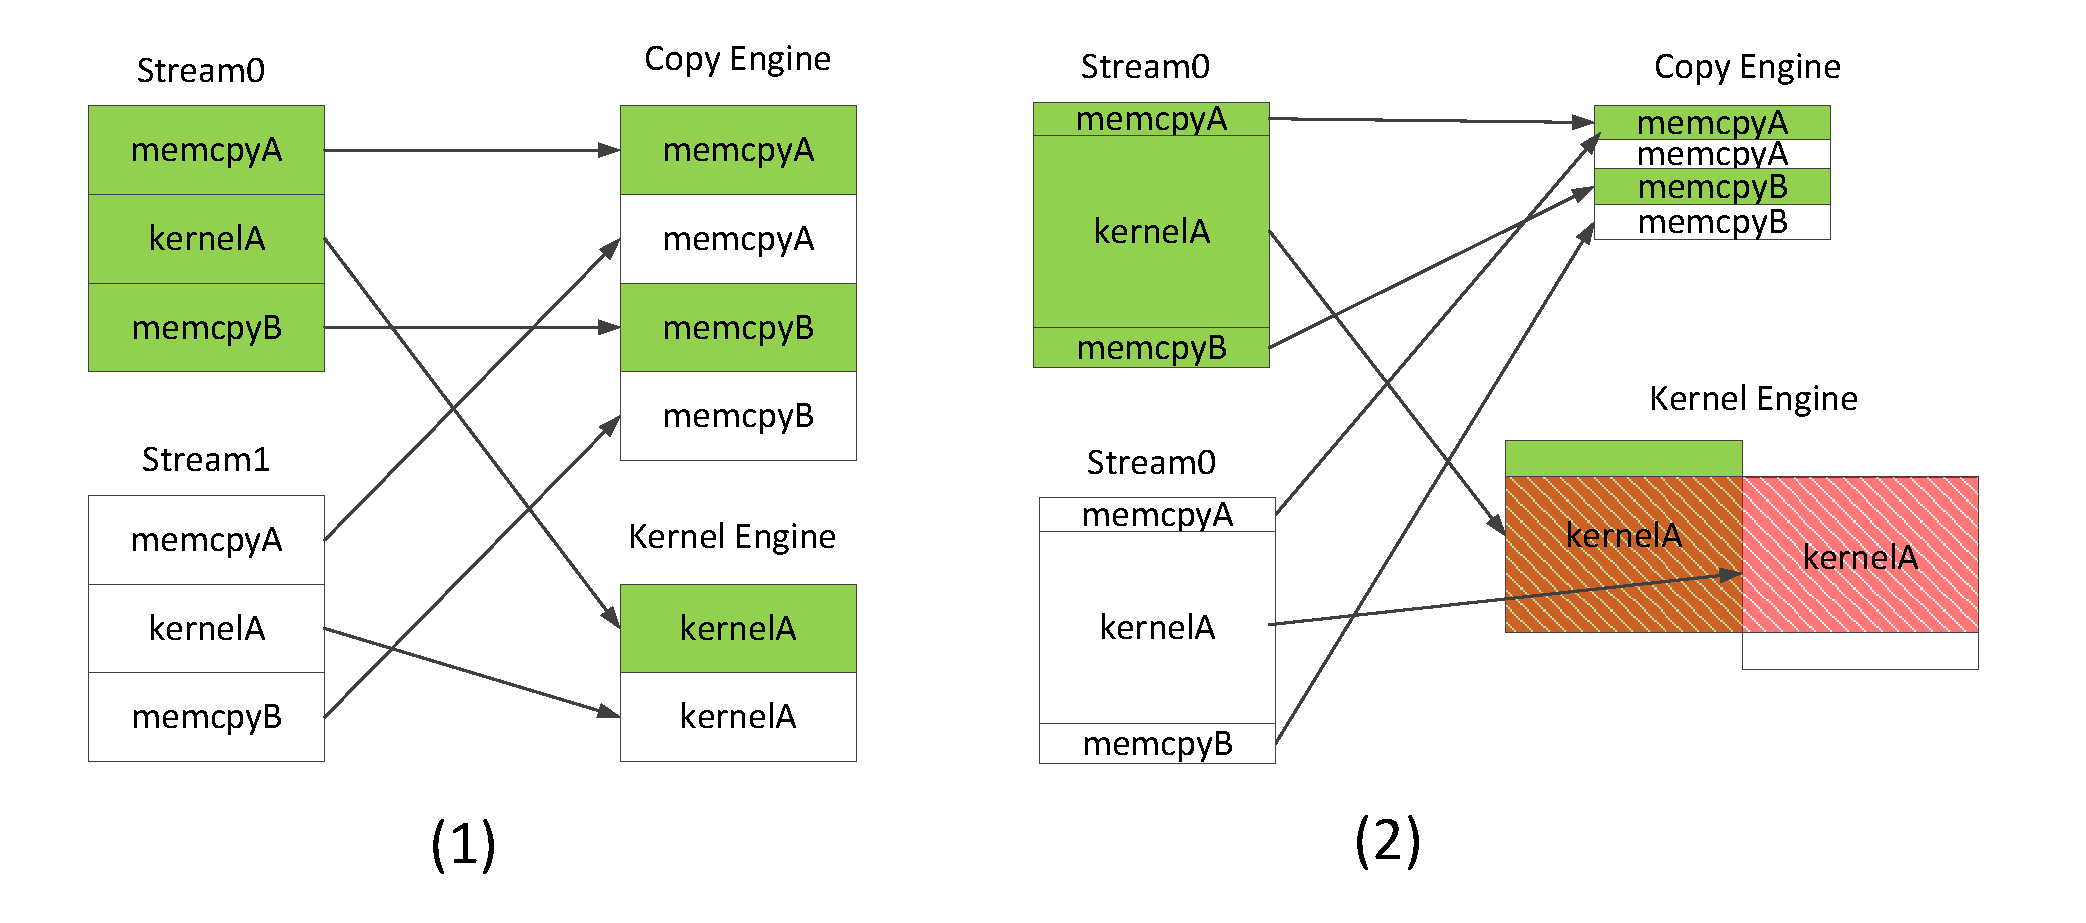
\includegraphics[width=1 \textwidth]{figures/flow.pdf}}
    \end{center}
  \caption{{\footnotesize{drk}}}
  \label{drk}
\end{figure*}
\subsection{本章总结}
本章简略介绍了GPU的体系架构和CUDA编程框架,说明了GPU的的强大计算能力和一些GPU程序设计上需要注意的问题。关于GPU架构和CUDA编程框架其实还有很多内容没有介绍,本章只介绍了一些本文会涉及到的GPU原理,为后面的3,4章介绍做铺垫。